%!TEX root=../GaugeCNNTheory.tex


\subsection{هم‌متغیری ایزومتری تبدیلات میدان کرنل و کانولوشن‌های \lr{GM}}
\label{sec:isometry_equivariance}


اکنون به بررسی این موضوع می‌پردازیم که تحت چه شرایطی تبدیلات میدان کرنل و کانولوشن‌های $\GM$ نسبت به عمل ایزومتری‌ها بر روی میدان‌های ویژگی هم‌متغیر هستند.
از آنجایی که عمل بر روی کلاف‌های بردار ویژگی \lr{G}-الحاقی فقط برای ایزومتری‌های حافظ \lr{G}-ساختار تعریف شده است، ما تمام گزاره‌ها را برای زیرگروه $\IsomGM \leq \IsomM$ یا زیرگروه‌های $\I \leq \IsomGM$ از آن فرمول‌بندی خواهیم کرد.
البته همیشه می‌توان گروه‌های ساختار $G\geq\O{d}$ را در نظر گرفت که برای آنها $\IsomGM = \IsomM$ است.


هم‌متغیری یک تبدیل میدان کرنل، و در نتیجه کانولوشن‌های $\GM$، به صورت زیر تعریف می‌شود:
\begin{dfn}[تبدیل میدان کرنل هم‌متغیر نسبت به ایزومتری]
\label{dfn:isometry_equivariance}
    فرض کنید ${\TK: \Gamma(\Ain) \to \Gamma(\Aout)}$ یک تبدیل میدان کرنل باشد.
    آنگاه گفته می‌شود که $\TK$ \emph{نسبت به عمل ایزومتری‌ها} در یک زیرگروه $\I \leq \IsomGM$ \emph{هم‌متغیر} است اگر با این عمل جابجا شود، یعنی اگر ویژگی زیر برقرار باشد:
    \begin{align}\label{eq:isom_equivariance_kernel_field_trafo_def}
        \TK \big( \phi\rhd\!f \big) \ =\ \phi\rhd\! \big( \TK(f) \big)
        \qquad \forall\ \ f\in\Gamma(\Ain), \ \ \phi\in \I
    \end{align}
    بر حسب یک نمودار، $\TK$ نسبت به ایزومتری‌ها در $\I$ هم‌متغیر است اگر
    \begin{equation}
    \begin{tikzcd}[column sep=70pt, row sep=35, font=\normalsize]
        \Gamma(\Ain)
            \arrow[r, "\TK"]
            \arrow[d, "\phi\,\rhd"']
        &
        \Gamma(\Aout)
            \arrow[d, "\phi\,\rhd"]
        \\
        \Gamma(\Ain)
            \arrow[r, "\TK"']
        &
        \Gamma(\Aout)
    \end{tikzcd}
    \end{equation}
    برای همه $\phi \in \I$ جابجا شود.
\end{dfn}
یک نمایش تصویری از این تعریف در شکل~\ref{fig:lizard_conv_egg} آورده شده است.
در بخش بعدی~\ref{sec:isometry_constraint} ما یک قید بر روی میدان‌های کرنل استخراج خواهیم کرد تا تبدیل میدان کرنل متناظر نسبت به ایزومتری هم‌متغیر باشد.
نتیجه‌ای که از نظر هندسی شهودی است و به دست می‌آوریم این است که خود میدان کرنل باید تحت عمل ایزومتری‌ها نامتغیر باشد، که این به معنای نوعی اشتراک‌گذاری وزن بر روی مدارهای ایزومتری است؛ به شکل~\ref{fig:isom_invariant_kernel_field_multiple_orbits} مراجعه کنید.
بخش~\ref{sec:isom_equiv_GM_conv} این بینش‌ها را به مورد خاص‌تر کانولوشن‌های $\GM$ و میدان‌های کرنل کانولوشنی $\GM$ اعمال می‌کند.
مشخص می‌شود که کانولوشن‌های $\GM$ به دلیل \lr{G}-هدایت‌پذیری کرنل الگوی خود، به طور خودکار نسبت به \emph{هر} ایزومتری در $\IsomGM$ هم‌متغیر هستند.








\subsubsection{هم‌متغیری ایزومتری تبدیلات میدان کرنل عمومی}
\label{sec:isometry_constraint}

نتیجه اصلی این بخش، قضیه~\ref{thm:isometry_equivariant_kernel_field_trafos}، بیان می‌کند که \emph{یک تبدیل میدان کرنل $\TK$ نسبت به ایزومتری هم‌متغیر است اگر و تنها اگر میدان کرنل زیربنایی آن $\K$ تحت ایزومتری‌ها نامتغیر باشد}.
برای معنادار کردن این گزاره، ما با تعریف رفتار تبدیلی میدان‌های کرنل هنگام عمل ایزومتری‌ها بر آنها شروع می‌کنیم.
\begin{dfn}[عمل ایزومتری بر روی میدان‌های کرنل]
\label{dfn:isometry_action_kernel_fields}
    فرض کنید $\K: \TM \to \Hom(\Ain,\Aout)$ یک میدان کرنل باشد.
    یک ایزومتری $\phi \in \IsomGM$ از طریق پیش‌ران میدان کرنل بر روی $\K$ عمل می‌کند:
    \begin{align}\label{eq:kernel_constraint_isom_full_1_persian}
        \dphiK \K\ :=\ \dphiHom \!\circ \K \circ \dphiTMinv \,.
    \end{align}
    به طور شهودی، این پیش‌ران میدان‌های کرنل را می‌توان به عنوان حرکت دادن کرنل‌های منفرد $\Kp$ در نقاط $p\in M$ در امتداد مدارهای گروه ایزومتری به $\phi(p)$ در نظر گرفت.
\end{dfn}
از آنجایی که میدان‌های کرنل به عنوان \lr{M}-مورفیسم‌های کلاف تعریف می‌شوند، یعنی $\piHom \K = \piTM$ را برآورده می‌کنند، پیش‌ران آنها تنها در صورتی خوش‌تعریف است که این ویژگی را حفظ کند.
این تضمین می‌شود زیرا پیش‌ران روی کلاف مماس و کلاف هومومورفیسم نگاشت‌های کلاف هستند که به ترتیب $\piTM \circ \dphiTM = \phi \circ \piTM$ (معادله~\eqref{cd:pushforward_TM}) و ${\piHom \circ \dphiHom = \phi \circ \piHom}$ (معادله~\eqref{cd:associated_bdl_automorphism}) را برآورده می‌کنند:
\begin{align}
    \piHom\, \dphiK \K
    \ &=\ \piHom\, \dphiHom \K\; \dphiTMinv \notag \\
    \ &=\ \phi\, \piHom\, \K\; \dphiTMinv \notag \\
    \ &=\ \phi\, \piTM\, \dphiTMinv \notag \\
    \ &=\ \phi\, \phiinv\, \piTM \notag \\
    \ &=\ \piTM
\end{align}
ما تعریف عمل ایزومتری را بر روی میدان‌های کرنل با یک نمودار جابجایی به تصویر می‌کشیم:
\begin{equation}
    \begin{tikzcd}[row sep=3.5em, column sep=2.8em]
        % ROW 1
        &[3.5ex] M & \\
        % ROW 2
        \TM  \arrow[ru, "\piTM"]
            \arrow[rr, pos=.56, "\dphiK \K"']
        & &
        \mkern-3mu
        \Hom(\Ain,\Aout)
            \arrow[lu, "\piHom"']
        \\
        % ROW 3
        \TM  \arrow[rd, "\piTM"']
            \arrow[rr, pos=.57, "\K"]
            \arrow[u, "\dphiTM"]
        & &
        \mkern-3mu
        \Hom(\Ain,\Aout)
            \arrow[ld, "\piHom"]
            \arrow[u, "\dphiHom"']
        \\
        % ROW 4
        & M 
            \arrow[uuu, rounded corners, to path={ 
                    -- ([xshift=-25ex]\tikztostart.west) 
                    --node[left, pos=.515]{\small$\phi$} ([xshift=-25ex]\tikztotarget.west) 
                    -- (\tikztotarget.west)
                    }]
        &
    \end{tikzcd}
    \quad
\end{equation}
بخش پایینی این نمودار میدان کرنل مستقل از مختصات $\K$ را از نمودار در معادله~\eqref{eq:kernel_bundle_map} نشان می‌دهد در حالی که بخش بالایی پیش‌ران آن $\dphiK \K = \dphiHom \!\circ \K \circ \dphiTMinv$ را توسط $\phi \in \IsomGM$ نشان می‌دهد.
جابجایی‌پذیری فلش سمت چپ، که تأیید می‌کند $\dphiK$ کرنل‌ها را از $p$ به $\phi(p)$ منتقل می‌کند، از این واقعیت ناشی می‌شود که $\dphiTM$ و $\dphiHom$ هر دو نگاشت‌های کلاف روی $\phi$ هستند.


ما با تعریف میدان‌های کرنل نامتغیر نسبت به ایزومتری ادامه می‌دهیم - یک نمایش تصویری در شکل~\ref{fig:isom_invariant_kernel_field_multiple_orbits} یافت می‌شود.
\begin{dfn}[میدان‌های کرنل نامتغیر نسبت به ایزومتری]
\label{dfn:isometry_invariant_kernel_fields}
    گفته می‌شود یک میدان کرنل $\K$ \emph{نامتغیر%
    \footnote{
        به جای گفتن اینکه $\K$ \emph{نامتغیر} است، می‌توان آن را \emph{هم‌متغیر} نامید زیرا
        $\dphiHom \!\circ \K \,=\ \K \circ \dphiTM \ \forall \phi\in\I$
        را برآورده می‌کند.
        به طور کلی، هر تابعی که نسبت به اعمال گروهی معینی بر روی دامنه و هم‌دامنه‌اش هم‌متغیر باشد، \emph{خودش} تحت پیش‌ترکیب و پس‌ترکیب با اعمال روی دامنه و هم‌دامنه‌اش مانند معادله~\eqref{eq:kernel_constraint_isom_full_1} نامتغیر است.
    }
    تحت ایزومتری‌ها} در $\I \leq \IsomGM$ است اگر قید $\dphiK \K = \K$ را برای همه $\phi \in \I$ برآورده کند.
    ما فضای میدان‌های کرنل نامتغیر نسبت به ایزومتری را با
    \begin{align}\label{eq:KIfull_def}
        \KIfull :=
            \pig\{\mkern2mu \K\mkern-2mu:\TM\to \Hom(\Ain,\Aout) \ \ \textup{هموار}\ \,\pig|\; 
            \piHom\!\circ\K = \piTM \,,\ \ \ 
            \dphiK \K  = \K \quad \forall \phi\in\I \,\pig\} \,.
    \end{align}
\end{dfn}
با نوشتن $\dphiK$، قید نامتغیر بودن به صورت زیر خوانده می‌شود:
\begin{align}\label{eq:kernel_constraint_isom_full_1}
    \dphiHom \!\circ \K \circ \dphiTMinv \,=\ \K \qquad \forall \phi\in\I \,,
\end{align}
که پس از بسط بیشتر $\dphiHom$ همانطور که در معادله~\eqref{eq:pushforward_Hom_def} تعریف شده است، به صورت زیر در می‌آید:
\begin{align}\label{eq:kernel_constraint_isom_full_2}
    \dphiAout
    \K \big(\dphiTMinv v\big) \ 
    \dphiAininv
    =\,
    \K(v) \qquad \forall\ v\in \TM,\ \ \forall \phi \in \I
\end{align}
به شباهت این قیود میدان کرنل در معادلات~\eqref{eq:kernel_constraint_isom_full_1} و~\eqref{eq:kernel_constraint_isom_full_2} با قید \lr{G}-هدایت‌پذیری بر روی کرنل‌های الگو در معادلات~\eqref{eq:G_steerable_space_in_dfn_Hom} و~\eqref{eq:G_steerable_space_in_dfn_classical} توجه کنید.
در واقع، هر دو قید ارتباط نزدیکی با هم دارند و تا حدی یکدیگر را ایجاب می‌کنند، همانطور که در بخش بعدی~\ref{sec:isom_equiv_GM_conv} در مورد کانولوشن‌های $\GM$ هم‌متغیر نسبت به ایزومتری نشان خواهیم داد.


\begin{SCfigure}
    \centering
    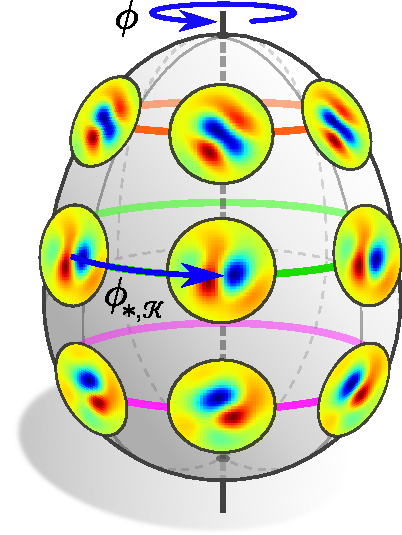
\includegraphics[width=.28\textwidth]{figures/isometry_egg_invariant_kernel.pdf}
    \hspace{10ex}
    \captionsetup{width=1.2\textwidth}
    \caption[]{\small
        نمایش تصویری یک میدان کرنل نامتغیر $\K$ برای حالت یک (زیر)گروه ایزومتری $\I = \SO2$.
        قید نامتغیر بودن مستلزم $\dphiK \K := \dphiHom \K \dphiTMinv = \K$ برای هر $\phi$ در $\I$ است.
        این ایجاب می‌کند که کرنل‌ها بر روی مدارهای $\I.p := \{\phi(p) \,|\, \phi \in \I\}$ عمل به اشتراک گذاشته شوند اما اجازه می‌دهد کرنل‌های متفاوتی بر روی مدارهای مختلف وجود داشته باشند.
        قضیه~\ref{thm:isometry_equivariant_kernel_field_trafos} اثبات می‌کند که میدان‌های کرنل نامتغیر و تبدیلات میدان کرنل هم‌متغیر یکدیگر را ایجاب می‌کنند.
        این به طور شهودی روشن است زیرا یک الگوی خاص در میدان ویژگی در $p\in M$ همان پاسخی را هنگامی که به $\phi(p)$ منتقل می‌شود برمی‌انگیزد، اگر و تنها اگر کرنل‌ها در هر دو نقطه منطبق باشند.
        برای انتخاب $\I = \O2$ به عنوان گروه ایزومتری، کرنل‌ها علاوه بر این باید یک قید بازتابی را برآورده کنند؛ به شکل~\ref{fig:isom_invariant_kernel_field_quotient} مراجعه کنید.
        \\\protect\rule{0ex}{2.ex}
        }
    \label{fig:isom_invariant_kernel_field_multiple_orbits}
\end{SCfigure}


قضیه زیر اثبات می‌کند که میدان‌های کرنلی که تحت ایزومتری‌ها نامتغیر هستند، در واقع متناظر با تبدیلات میدان کرنل هم‌متغیر نسبت به ایزومتری هستند:
\begin{thm}[تبدیل میدان کرنل هم‌متغیر $\Leftrightarrow$ میدان کرنل نامتغیر]
\label{thm:isometry_equivariant_kernel_field_trafos}
 \ یک تبدیل میدان کرنل $\TK: \Gamma(\Ain)\to \Gamma(\Aout)$ نسبت به ایزومتری‌ها در $\I \leq \IsomGM$ طبق تعریف~\ref{dfn:isometry_equivariance} هم‌متغیر است اگر و تنها اگر
 میدان کرنل زیربنایی $\K$ تحت ایزومتری‌ها طبق تعریف~\ref{dfn:isometry_invariant_kernel_fields} نامتغیر باشد، یعنی،
    \begin{align}
        \TK(\phi \rhd f) \,=\, \phi \rhd \TK(f)
        \quad\forall\; \phi \in \I\,,\ f\in\Gamma(\Ain)
        \quad \Longleftrightarrow \quad
        \dphiK \K = \K
        \quad\forall\, \phi \in \I
    \end{align}
\end{thm}
\begin{proof}
    برای اثبات این قضیه، ما تبدیلات میدان کرنل و پیش‌ران‌های میدان ویژگی را در هر دو طرف شرط هم‌متغیری ایزومتری در معادله~\eqref{eq:isom_equivariance_kernel_field_trafo_def} می‌نویسیم.
    گزاره پس از چند دستکاری جبری از مقایسه هر دو طرف به دست می‌آید.

    ما با سمت راست معادله~\eqref{eq:isom_equivariance_kernel_field_trafo_def} شروع می‌کنیم:
    \begin{align}
        \big[ \phi \rhd \TK(f) \big](p)
        \ &\overset{(1)}{=}\ \ 
            \dphiAout \big[ \TK(f) \big] \big( \phi^{-1}(p) \big) \notag \\[1ex]
        \ &\overset{(2)}{=}\ \ 
            \dphiAout \mkern-8mu
            \int\limits_{T_{\!\phiinv\mkern-1mu(p)}\mkern-2muM}\!\!
            \mkern-6mu \K(v) \ 
            \big[\mkern-2mu \Expsphiinvpf \mkern1mu\big] (v)
            \,\ dv \notag \\
        \ &\overset{(3)}{=}\ \ 
            \dphiAout \mkern-8mu
            \int\limits_{T_{\!\phiinv\mkern-1mu(p)}\mkern-2muM}\!\!
            \mkern-6mu \K(v) \ 
            \dphiAin^{-1} \big[\mkern-2mu \Expsp\! \big(\phi \rhd f\big) \mkern1mu\big] \big( \dphiTM (v) \big)
            \,\ dv \notag \\
        \ &\overset{(4)}{=}\ \ 
            \int\limits_{\TpM}
            \dphiAout
            \K\big( \dphiTM^{-1} \tilde{v} \big) \ 
            \dphiAin^{-1} \big[\mkern-2mu \Expsp\! \big(\phi \rhd f\big) \mkern1mu\big] (\tilde{v})
            \,\ d\tilde{v} \notag \\
        \ &\overset{(5)}{=}\ \ 
            \int\limits_{\TpM}
            \big[ \dphiHom \K\, \dphiTM^{-1} \big] (\tilde{v}) \ 
            \big[\mkern-2mu \Expsp\! \big(\phi \rhd f\big) \mkern1mu\big] (\tilde{v})
            \,\ d\tilde{v} \notag \\
        \ &\overset{(6)}{=}\ \ 
            \int\limits_{\TpM}
            \big[ \dphiK \K \big] (\tilde{v}) \ 
            \big[\mkern-2mu \Expsp\! \big(\phi \rhd f\big) \mkern1mu\big] (\tilde{v})
            \,\ d\tilde{v}
    \end{align}
    مراحل (۱) و (۲) عمل ایزومتری $\rhd$ را بر روی میدان‌های ویژگی (تعریف~\ref{dfn:isometry_pushforward}) و تبدیل میدان کرنل (تعریف~\ref{dfn:kernel_field_trafo}) بسط می‌دهند.
    قانون تبدیل پول‌بک منتقل‌کننده میدان در قضیه~\ref{thm:transporter_pullback_isometry_action}، که به نامتغیر بودن اتصال \lr{G}-سازگار نسبت به $\IsomGM$ متکی است، مرحله (۳) را توجیه می‌کند.
    مرحله (۴) $v$ را با $\tilde{v} = \dphiTM v$ جایگزین می‌کند.
    از آنجایی که $\phi$ یک ایزومتری است، تغییر حجم برابر با ۱ است.
    مراحل (۵) و (۶) عمل پیش‌ران کرنل $\dphiK$ را شناسایی می‌کنند، تعریف~\ref{dfn:isometry_action_kernel_fields}.
    گزاره حاصل کاملاً شهودی است:
    یک تبدیل خروجی تبدیل میدان کرنل متناظر با یک تبدیل همزمان ورودی \emph{و} میدان کرنل آن است.

    نوشتن سمت چپ به دست می‌دهد:
    \begin{align}
        \big[ \TK \big(\phi \rhd f\big) \big](p)
        \ =\ \int\limits_{\TpM}
                \K(v) \ 
                \big[\mkern-2mu \Expsp\!\big( \phi\rhd f\big) \mkern1mu\big] (v)
                \,\ dv \,,
    \end{align}
    که \emph{تا} تبدیل میدان کرنل با سمت راست معادل است.

    هم‌متغیری ایزومتری مستلزم آن است که هر دو عبارت برای میدان‌های دلخواه $f\in\Gamma(\Ain)$، نقاط $p\in M$ و ایزومتری‌های $\phi\in\I$ موافق باشند.
    این حالت اگر و تنها اگر $\dphiK \K = \K$ برای هر $\phi \in \I$ برقرار باشد، یعنی اگر میدان کرنل تحت عمل ایزومتری‌ها نامتغیر باشد، برقرار است.
\end{proof}
توجه داشته باشید که این اثبات در (یک \lr{G}-اطلس از) بدیهی‌سازی‌های محلی بسیار دشوار بود.
توصیف سراسری و مستقل از مختصات تبدیلات میدان کرنل امکان یک اثبات ساده را بدون نگرانی از اینکه ایزومتری‌ها ویژگی‌ها را بین بدیهی‌سازی‌های محلی مختلف منتقل کنند، فراهم می‌کند.


در این مرحله ما می‌توانستیم با بررسی بیشتر میدان‌های کرنل نامتغیر نسبت به ایزومتری ادامه دهیم:
از آنجایی که قید نامتغیر بودن ایجاب می‌کند که کرنل‌ها بر روی مدارهای گروه ایزومتری به اشتراک گذاشته شوند، توصیف کل میدان کرنل بر روی کل منیفلد زائد است.
بنابراین امکان کاهش توصیف چنین میدان‌های کرنلی به میدان‌های کرنل بر روی فضاهای خارج‌قسمتی وجود دارد.
از آنجایی که این تحلیل برای اثبات هم‌متغیری ایزومتری کانولوشن‌های $\GM$ لازم نیست و به برخی تعاریف فنی نیاز دارد، ما آن را به بخش~\ref{sec:quotient_kernel_fields} موکول می‌کنیم.




















\subsubsection{هم‌متغیری ایزومتری کانولوشن‌های \lr{GM}}
\label{sec:isom_equiv_GM_conv}

به یاد بیاورید که کانولوشن‌های $\GM$ (تعریف~\ref{dfn:coord_free_conv}) به عنوان تبدیلات میدان کرنل خاص با میدان‌های کرنل کانولوشنی $\GM$ (تعریف~\ref{dfn:conv_kernel_field}) تعریف شدند.
بنابراین نتایج مربوط به هم‌متغیری ایزومتری تبدیلات میدان کرنل بلافاصله به کانولوشن‌های $\GM$ نیز اعمال می‌شود.
با این حال، علاوه بر قید نامتغیر بودن ایزومتری در معادله~\eqref{eq:kernel_constraint_isom_full_1}، میدان‌های کرنل کانولوشنی $\GM$ باید قید \lr{G}-هدایت‌پذیری را بر روی کرنل الگو از معادله~\eqref{eq:G_steerable_space_in_dfn_Hom} برآورده کنند و وزن‌ها را طبق معادله~\eqref{eq:conv_kernel_field_def_ptwise} بر روی \lr{G}-ساختار به اشتراک بگذارند.
برای اینکه کانولوشن $\GM$ نسبت به ایزومتری هم‌متغیر باشد، همه این قیود باید به طور همزمان برآورده شوند.
به طور شهودی، این ایجاب می‌کند که اشتراک‌گذاری وزن کانولوشنی با اشتراک‌گذاری وزن القا شده از ایزومتری بر روی مدارها موافق باشد.
خوشبختانه مشخص می‌شود که این به طور خودکار برای ایزومتری‌های مورد نظر صادق است:
کانولوشن‌های $\GM$ وزن‌ها را بر روی \lr{G}-ساختار به اشتراک می‌گذارند و ایزومتری‌ها در $\IsomGM$ \lr{G}-ساختار را حفظ می‌کنند به طوری که \emph{میدان‌های کرنل کانولوشنی $\GM$ تضمین شده‌اند که نسبت به $\IsomGM$ نامتغیر باشند}.
در مختصات، این در تبدیلات پیمانه القا شده از $\IsomGM$ یعنی $g_\phi^{A\widetilde{A}}(p)$ که در گروه ساختار $G$ مقدار می‌گیرند، منعکس می‌شود، به طوری که آنها توسط \lr{G}-هدایت‌پذیری کرنل‌های الگو حذف می‌شوند.


برای دقیق‌تر کردن این استدلال‌ها، یک کانولوشن $\GM$ یعنی $K\star: \Gamma(\Ain) \to \Gamma(\Aout)$ را با یک کرنل \lr{G}-هدایت‌پذیر $K \in \KG$ در نظر بگیرید، که طبق تعریف~\ref{dfn:coord_free_conv} فقط تبدیل میدان کرنل $\TKK$ با میدان کرنل کانولوشنی $\GM$ یعنی $\KK$ است.
طبق قضیه~\ref{thm:isometry_equivariant_kernel_field_trafos}، کانولوشن $\GM$ بنابراین دقیقاً زمانی نسبت به $\IsomGM$ هم‌متغیر است که $\KK$ نسبت به $\IsomGM$ نامتغیر باشد، یعنی زمانی که $\dphiK \KK = \dphiHom \circ \KK \circ \dphiTMinv = \KK$ را برای هر $\phi \in \IsomGM$ برآورده کند.
این قید بر روی کل میدان کرنل به طور معادل با مجموعه‌ای از قیود بر روی کرنل‌های کانولوشن منفرد که میدان را تشکیل می‌دهند، بیان می‌شود:
\begin{align}\label{eq:KK_constraint_ptwise_abstract}
    \dphiHom \circ \KKp \circ \dphiTMinv \ &=\ \KKphip \qquad \forall\ p\in M,\ \ \phi \in \IsomGM
\end{align}
با در نظر گرفتن یک نقطه خاص $p\in M$، ما پیمانه‌های دلخواه $\widetilde{A}$ را در $p$ و $A$ را در $\phi(p)$ از \lr{G}-اطلس انتخاب می‌کنیم.
میدان کرنل کانولوشنی $\GM$ طبق تعریف~\ref{dfn:conv_kernel_field} در $p$ و $\phi(p)$ به صورت زیر داده می‌شود:
\begin{align}
    \KKp    := \big(\psiHomp^{\widetilde{A}} \big)^{-1} \circ \frac{K}{\sqrt{|\eta_p^{\widetilde{A}}|}} \circ \psiTMp^{\widetilde{A}}
    \qquad \textup{و} \qquad
    \KKphip := \big(\psiHomphip^A           \big)^{-1} \circ \frac{K}{\sqrt{|\eta_{\phi(p)}^A|}}      \circ \psiTMphip^A \,.
\end{align}
با جایگذاری این عبارات در قید در معادله~\eqref{eq:KK_constraint_ptwise_abstract} برای $p$ ثابت و شناسایی $\dphiHom \big(\psiHomp^{\widetilde{A}} \big)^{-1}$ با $\big( \psiHomp^{\widetilde{A}}\, \dphiHom^{-1}  \big)^{-1}$ به دست می‌آوریم:
\begin{align}\label{eq:GM-conv_kernel_field_isom_invariance_1}
    \big( \psiHomp^{\widetilde{A}}\, \dphiHom^{-1}  \big)^{-1} \circ \frac{K}{\sqrt{|\eta_p^{\widetilde{A}}|}} \circ \psiTMp^{\widetilde{A}}\, \dphiTMinv
    \,\ &=\,\ \big(\psiHomphip^A \big)^{-1} \circ \frac{K}{\sqrt{|\eta_{\phi(p)}^A|}} \circ \psiTMphip^A
    \qquad \forall\ \phi \in \IsomGM
\end{align}
بنابراین هم‌متغیری ایزومتری برقرار خواهد بود اگر اشتراک‌گذاری وزن از طریق پیمانه‌های القا شده از ایزومتری $\psidotp^{\widetilde{A}} \dphidot$ با اشتراک‌گذاری وزن از طریق پیمانه‌های اصلی $\psidotphip^A$ از $\phi(p)$ موافق باشد.
به یاد بیاورید که پیمانه‌های القا شده از ایزومتری طبق قضیه~\ref{thm:isom_GM_in_coords} برای ایزومتری‌ها در $\IsomGM$ تضمین شده‌اند که با \lr{G}-اطلس‌ها (از کلاف متناظر) سازگار باشند.
همانطور که در معادله~\eqref{eq:arbitrariness_gauge_GM_kernel_field_def} نشان داده شده است، انتخاب خاص پیمانه، که کرنل الگوی \lr{G}-هدایت‌پذیر نسبت به آن جهت‌دهی می‌شود، بی‌اهمیت است، تا زمانی که پیمانه‌ها \lr{G}-سازگار باشند.
از آنجایی که همه استخراج‌ها از نقطه انتخاب شده $p$ و انتخاب خاص پیمانه‌ها مستقل بودند، این ایجاب می‌کند که کانولوشن‌های $\GM$ بنا به طراحی تضمین شده‌اند که نسبت به $\IsomGM$ هم‌متغیر باشند.


برای به دست آوردن شهود بهتر برای این نتیجه، ارزش دارد که تبدیلات پیمانه القایی و با مقدار در \lr{G} یعنی $g_\phi^{A\widetilde{A}}(p)$ را صریح کنیم.
برای این منظور، توجه داشته باشید که جابجایی‌پذیری نمودارها در معادلات~\eqref{cd:pushforward_A_coord} و~\eqref{cd:pushforward_TM_coord} ایجاب می‌کند
$\psiHomp^{\widetilde{A}}\, \dphiHominv = \rhoHom\big( g_\phi^{A\widetilde{A}}(p) \big)^{-1} \psiHomphip^A$ و
$\psiTMp^{\widetilde{A}}\,  \dphiTMinv  =         \big( g_\phi^{A\widetilde{A}}(p) \big)^{-1} \psiTMphip^A$.
با جایگذاری این عبارات مختصاتی در قید در معادله~\eqref{eq:GM-conv_kernel_field_isom_invariance_1} به این الزام می‌رسیم که
\begin{align}\label{eq:GM-conv_kernel_field_isom_invariance_2}
    \Big(\mkern-1.5mu \rhoHom\big( g_\phi^{A\widetilde{A}}(p) \big)^{-1} \psiHomphip^A \mkern-1.5mu\Big)^{-1}
    \!\circ \frac{K}{\sqrt{|\eta_p^{\widetilde{A}}|}} \circ \big( g_\phi^{A\widetilde{A}}(p) \big)^{-1} \psiTMphip^A
    \ &=\ \big(\psiHomphip^A \big)^{-1} \!\circ \frac{K}{\sqrt{|\eta_{\phi(p)}^A|}} \circ \psiTMphip^A
\end{align}
باید برای هر ایزومتری $\phi$ در $\IsomGM$ برقرار باشد.
با بسط دادن معکوس در سمت چپ، با استفاده از اینکه
${\sqrt{|\eta_p^{\widetilde{A}}|} \,= \sqrt{|\eta_{\phi(p)}^A|} \cdot \big|\mkern-2mu \det g^{A\widetilde{A}}_\phi(p) \big|}$
و حذف پیمانه‌ها، که ممکن است زیرا آنها ایزومورفیسم هستند، ما به قید زیر می‌رسیم:
\begin{align}\label{eq:GM_conv_isom_constraint_coords}
    \frac{1}{\big|\mkern-2mu \det g^{A\widetilde{A}}_\phi(p) \big|} \,
    \rhoHom\Big(g^{A\widetilde{A}}_\phi(p)\Big) \circ K \circ \Big(g^{A\widetilde{A}}_\phi(p)\Big)^{-1} \ =\ K
    \qquad \forall\ \phi \in \IsomGM \,,
\end{align}
که \emph{دقیقاً} شبیه قید کرنل \lr{G}-هدایت‌پذیر بر روی $K$ از تعریف~\ref{dfn:G-steerable_kernel_def_43} است.
به یاد بیاورید که تبدیلات پیمانه القا شده از ایزومتری $g_\phi^{A\widetilde{A}}(p)$ طبق قضیه~\ref{thm:isom_GM_in_coords} تضمین شده‌اند که اگر $\phi$ عنصری از $\IsomGM$ باشد، با مقدار در \lr{G} باشند.
بنابراین قید در معادله~\eqref{eq:GM_conv_isom_constraint_coords} همیشه با \lr{G}-هدایت‌پذیری $K$ برآورده می‌شود.

نتایج استخراج شده در مورد نامتغیر بودن میدان‌های کرنل کانولوشنی $\GM$ یعنی $\KK$ نسبت به $\IsomGM$ به طور خلاصه با این گزاره خلاصه می‌شوند که نمودار زیر تضمین شده است که اگر $K$ \lr{G}-هدایت‌پذیر باشد و اگر $\phi \in \IsomGM$ حافظ \lr{G}-ساختار باشد، جابجایی‌پذیر است:
\begin{equation}
    \begin{tikzcd}[row sep=4.em, column sep=5.5em] %,
        % ROW 1
        & &[-2.7em] U^A &[-2.7em] & \\[-1em]
        % ROW 2
        U^A \mkern-2mu\times\mkern-1mu \R^d
            \arrow[rrrr, rounded corners, to path={ 
                    -- ([yshift=15ex]\tikztostart.north) 
                    --node[above]{\small
                            $\id\times \pig( \rhoHom\big(g'^{A\widetilde{A}}_\phi\big) \circ K \big/\mkern-2mu \sqrt{|\eta^A|} \circ \big(g'^{A\widetilde{A}}_\phi\big)^{-1} \pig)$
                            } ([yshift=15ex]\tikztotarget.north) 
                    -- (\tikztotarget.north)
                    }]
        &
        \,\piTM^{-1}\big(U^A\big)
            \arrow[ru, "\piTM"]
            \arrow[rr, "\dphiK \KK"']
            \arrow[l, "\PsiTM^A"']
        & &
        \piHom^{-1}\big(U^A\big)
            \arrow[lu, "\piHom"']
            \arrow[r, "\PsiHom^A"]
        &
        U^A \mkern-2mu\times\mkern-1mu \R^{\cout\times\cin}
        \\
        % ROW 3
        U^{\widetilde{A}} \mkern-2mu\times\mkern-1mu \R^d
            \arrow[u, "\phi \times g_\phi^{A\widetilde{A}}\cdot"']
            \arrow[rrrr, rounded corners, to path={ 
                    -- ([yshift=-15ex]\tikztostart.south) 
                    --node[below]{\small$\id\times K \big/\mkern-2mu \sqrt{|\eta^{\widetilde{A}}|}$} ([yshift=-15ex]\tikztotarget.south) 
                    -- (\tikztotarget.south)
                    }]
        &
        \piTM^{-1}\big(U^{\widetilde{A}}\big)
            \arrow[rd, "\piTM"']
            \arrow[rr, "\KK"]
            \arrow[u, "\dphiTM"]
            \arrow[l, "\PsiTM^{\widetilde{A}}"]
        & &
        \piHom^{-1}\big(U^{\widetilde{A}}\big)
            \arrow[ld, "\piHom"]
            \arrow[u, "\dphiHom"']
            \arrow[r, "\PsiHom^{\widetilde{A}}"']
        &
        U^{\widetilde{A}} \mkern-2mu\times\mkern-1mu \R^{\cout\times\cin}
            \arrow[u, "\phi \times \rhoHom\big(g_\phi^{A\widetilde{A}}\big)"]
        \\[-1em]
        % ROW 4
        & & U^{\widetilde{A}}
        & &
    \end{tikzcd}
\end{equation}
در اینجا ما پول‌بک $g_\phi'^{A\widetilde{A}} := g_\phi^{A\widetilde{A}} \circ \phi^{-1} : U^A \to G$ از مختصاتی‌سازی پیش‌ران ایزومتری را از $U^{\widetilde{A}}$ به $U^A$ برای راحتی نوشتاری تعریف کردیم.


همراه با قضیه~\ref{thm:isometry_equivariant_kernel_field_trafos}، نامتغیر بودن میدان‌های کرنل کانولوشنی $\GM$ نسبت به $\IsomGM$ هم‌متغیری کانولوشن‌های $\GM$ نسبت به $\IsomGM$ را ایجاب می‌کند:
\begin{thm}[هم‌متغیری ایزومتری کانولوشن‌های $\GM$]
\label{thm:isom_equiv_GM_conv}
    یک کانولوشن $\GM$ یعنی $K\star: \Gamma(\Ain)\to \Gamma(\Aout)$ با یک کرنل \lr{G}-هدایت‌پذیر $K\in\KG$ نسبت به تمام ایزومتری‌های حافظ \lr{G}-ساختار $\phi \in \IsomGM$ هم‌متغیر است، یعنی،
    \begin{align}
        K \star \big( \phi \rhd f \big) \ =\ 
        \phi \rhd \big( K \star  f \big)
        \qquad \forall\ \ f\in\Gamma(\Ain), \ \ \phi\in \IsomGM \,.
    \end{align}
    بنابراین نمودار زیر برای هر $\phi \in \IsomGM$ جابجا می‌شود:
    \begin{equation}
    \begin{tikzcd}[column sep=60pt, row sep=35, font=\normalsize]
        \Gamma(\Ain)
            \arrow[r, "K\star"]
            \arrow[d, "\phi\,\rhd\,"']
        &
        \Gamma(\Aout)
            \arrow[d, "\,\phi\,\rhd"]
        \\
        \Gamma(\Ain)
            \arrow[r, "K\star"']
        &
        \Gamma(\Aout)
    \end{tikzcd}
    \end{equation}
\end{thm}
\begin{proof}
    اثبات در بحث قبل از قضیه ارائه شد.
\end{proof}



با استخراج این نتیجه کلی در مورد کانولوشن‌های $\GM$، ما اکنون برخی موارد خاص را برای انتخاب‌های خاص از گروه‌های ساختار $G$ مورد بحث قرار می‌دهیم.
اولاً، برای گروه‌های ساختار متعامد $G=\O{d}$ (یا ابرگروه‌های آن)، کانولوشن با \emph{هر} ایزومتری جابجا می‌شود:
\begin{thm}[هم‌متغیری کامل ایزومتری کانولوشن‌های $\OM$]
\label{thm:Od_equiv_OM_conv}
    کانولوشن‌های $\OM$ نسبت به عمل \emph{هر} ایزومتری $\phi \in \IsomM$ بر روی میدان‌های ویژگی هم‌متغیر هستند.
    به طور کلی‌تر، هر کانولوشن $\GM$ برای \lr{G}-ساختارها با گروه‌های ساختار $G\geq\O{d}$ کاملاً نسبت به ایزومتری هم‌متغیر است.
\end{thm}
\begin{proof}
    گزاره از قضیه~\eqref{thm:isom_equiv_GM_conv} با مشاهده اینکه $\IsomGM = \IsomM$ برای گروه‌های ساختار $G \geq \O{d}$ تضمین شده است، به دست می‌آید.
    دومی در معادله~\eqref{eq:isomM_isomOM} مورد بحث قرار گرفت.
\end{proof}
این نتیجه اساساً به این واقعیت متکی است که ایزومتری‌ها به عنوان آن زیرگروهی از دیفئومورفیسم‌ها بر روی $M$ تعریف می‌شوند که خودریختی‌های $\O{d}$-ساختار را القا می‌کنند.
به بیان کمتر انتزاعی، $\IsomM$ بنا به تعریف آن زیرگروهی از دیفئومورفیسم‌ها است که به متریک ریمانی $\eta$ از $M$ احترام می‌گذارد و $\O{d}$-ساختار متناظر $\OM$ اطلاعاتی معادل با متریک است.


بر روی منیفلدهای ریمانی جهت‌پذیر، می‌توان علاوه بر این یک جهت (دست‌گردی قاب) را انتخاب کرد، که همراه با متریک یک $\SO{d}$-ساختار $\SOM$ را تعریف می‌کند.
ایزومتری‌های متناظر که به خودریختی‌های ساختار $\SO{d}$ بالابر می‌شوند، ایزومتری‌های حافظ جهت در $\IsomplusM$ هستند.
\begin{thm}[هم‌متغیری $\IsomplusM$ کانولوشن‌های $\SOM$]
\label{thm:SOd_equiv_SOM_conv}
    کانولوشن‌های $\SOM$ نسبت به عمل ایزومتری‌های حافظ جهت $\phi \in \IsomplusM$ بر روی میدان‌های ویژگی هم‌متغیر هستند.
\end{thm}
\begin{proof}
    این نتیجه از قضیه~\eqref{thm:isom_equiv_GM_conv} با مشاهده اینکه $\IsomSOM = \IsomplusM$ به دست می‌آید.
\end{proof}
به عنوان مثال، یک کانولوشن $\SOM$ برای $M=\R^2$ که متناظر با شکل~\ref{fig:SO2_structure_SE2} است، نسبت به عمل گروه اقلیدسی ویژه $\Isom_+(\R^2) = \SE2$ هم‌متغیر است.
به طور مشابه، یک کانولوشن $\SOM$ برای $M=S^2$ که متناظر با شکل~\ref{fig:SO2_structure_SO3} است، نسبت به دوران با $\Isom_+(S^2) = \SO3$ هم‌متغیر است.


توجه داشته باشید که نتایج قضایای~\ref{thm:Od_equiv_OM_conv} و~\ref{thm:SOd_equiv_SOM_conv} فقط به گروه ساختار $G$ بستگی دارند اما به انتخاب خاص \lr{G}-ساختار بستگی ندارند.
برای زیرگروه‌های $G$ از $\O{d}$ (یا $\SO{d}$) مسائل پیچیده‌تر می‌شوند.
در این موارد، زیرگروه‌های $\IsomGM$ از $\IsomM$ به نشاندن خاص \lr{G}-ساختار $\GM$ در $\FM$ بستگی دارند.
این برای $G=\{e\}$ در شکل~\ref{fig:frame_field_automorphism} به تصویر کشیده شد.
به طور خاص، شکل~\ref{fig:frame_field_automorphism_1} $\{e\}$-ساختار کانونی $\R^2$ را نشان می‌دهد که کاملاً نسبت به انتقال هم‌متغیر است، یعنی $\IsomeM = \Trans_2 := (\R^2,+)$.
در مقابل، شکل~\ref{fig:frame_field_automorphism_2} یک $\{e\}$-ساختار از $\R^2$ را نشان می‌دهد که فقط در امتداد یک محور نسبت به انتقال هم‌متغیر است به طوری که $\IsomeM \cong \Trans_1 := (\R,+)$.
از دیدگاه شبکه‌های کانولوشنی این نتیجه بسیار شهودی است:
کرنل‌های $\{e\}$-هدایت‌پذیر در این مثال‌ها بدون قید هستند، یعنی کرنل‌های کانولوشن مرسوم هستند.
بنابراین آنها به طور کلی هیچ اطلاعاتی در مورد پاسخ‌های خود هنگام اعمال نسبت به قاب‌های مرجع تبدیل‌شده با پیمانه حمل نمی‌کنند.
از آنجایی که قاب‌ها، و بنابراین کرنل‌ها، در شکل~\ref{fig:frame_field_automorphism_2} در جهت «چپ-راست» به طور متفاوتی چرخانده شده‌اند، پاسخ‌های کرنل هنگام انتقال یک سیگنال در آن جهت به طور غیرقابل پیش‌بینی تغییر می‌کنند.
اگر کرنل‌های الگو، با این حال، $\SO2$-هدایت‌پذیر بودند، می‌توانستند چرخش قاب‌ها را در نظر بگیرند.
این حالت متناظر با وضعیت در شکل~\ref{fig:SO2_structure_SE2} است، یعنی یک کانولوشن $\SOM$.